%%%%%%%%%%%%%%%%%%%%%%%%%%%%%%%%%%%%%%%%%%%%%%%%%%%%%%%%%%%%%%%%%%%%%%
%%%%                                                              %%%%
%%%% WISHBONE SD Card Controller IP Core                          %%%%
%%%%                                                              %%%%
%%%% introduction.tex                                             %%%%
%%%%                                                              %%%%
%%%% This file is part of the WISHBONE SD Card                    %%%%
%%%% Controller IP Core project                                   %%%%
%%%% http://opencores.org/project,sd_card_controller              %%%%
%%%%                                                              %%%%
%%%% Description                                                  %%%%
%%%% documentation 'Introduction' chapter                         %%%%
%%%%                                                              %%%%
%%%% Author(s):                                                   %%%%
%%%%     - Marek Czerski, ma.czerski@gmail.com                    %%%%
%%%%                                                              %%%%
%%%%%%%%%%%%%%%%%%%%%%%%%%%%%%%%%%%%%%%%%%%%%%%%%%%%%%%%%%%%%%%%%%%%%%
%%%%                                                              %%%%
%%%% Copyright (C) 2013 Authors                                   %%%%
%%%%                                                              %%%%
%%%% This source file may be used and distributed without         %%%%
%%%% restriction provided that this copyright statement is not    %%%%
%%%% removed from the file and that any derivative work contains  %%%%
%%%% the original copyright notice and the associated disclaimer. %%%%
%%%%                                                              %%%%
%%%% This source file is free software; you can redistribute it   %%%%
%%%% and/or modify it under the terms of the GNU Lesser General   %%%%
%%%% Public License as published by the Free Software Foundation; %%%%
%%%% either version 2.1 of the License, or (at your option) any   %%%%
%%%% later version.                                               %%%%
%%%%                                                              %%%%
%%%% This source is distributed in the hope that it will be       %%%%
%%%% useful, but WITHOUT ANY WARRANTY; without even the implied   %%%%
%%%% warranty of MERCHANTABILITY or FITNESS FOR A PARTICULAR      %%%%
%%%% PURPOSE. See the GNU Lesser General Public License for more  %%%%
%%%% details.                                                     %%%%
%%%%                                                              %%%%
%%%% You should have received a copy of the GNU Lesser General    %%%%
%%%% Public License along with this source; if not, download it   %%%%
%%%% from http://www.opencores.org/lgpl.shtml                     %%%%
%%%%                                                              %%%%
%%%%%%%%%%%%%%%%%%%%%%%%%%%%%%%%%%%%%%%%%%%%%%%%%%%%%%%%%%%%%%%%%%%%%%
\section{Introduction}
\label{sec:introduction}

    This document descripes the multimedia card (MMC) / secure digital (SD) card controller ip core - \textit{Wishbone SD Card Controller IP Core}.

    \subsection{Purpose of the IP core}
    \label{sec:purpose}

    The \textit{Wishbone SD Card Controller IP Core} is an MMC/SD communication controller designed to be used in a System-on-Chip (Fig. \ref{img:ip_core}).
    The IP core provides a simple interface for any MCU which utilizes the Wishbone bus. Communications between the MMC/SD card controller and MMC/SD card 
    are performed according to the MMC/SD protocol.
    
    \begin{figure}[H]
        \centering
        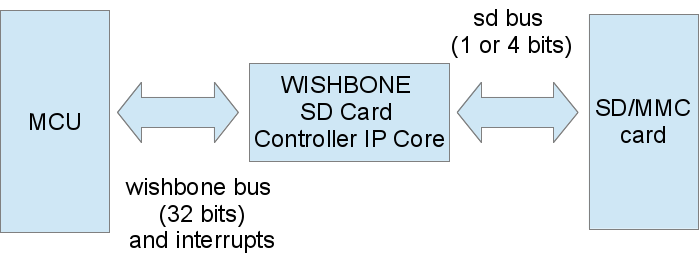
\includegraphics[width=11cm]{../bin/ip_core.png}
        % ip_core.png: 384x469 pixel, 96dpi, 10.16x12.41 cm, bb=
        \caption{SoC with SD Card IP core}
        \label{img:ip_core}
    \end{figure}
    
    \subsection{Features}
    \label{sec:fetures}
    The MMC/SD card controller provides following features:
    
    \begin{itemize}
     \item 1- or 4-bit MMC/SD mode (does not support SPI mode),
     \item 32-bit Wishbone interface,
     \item DMA engine for data transfers,
     \item Interrupt generation on completion of data and command transactions,
     \item Configurable data transfer block size,
     \item Support for any command code (including multiple data block tranfser),
     \item Support for R1, R1b, R2(136-bit), R3, R6 and R7 responses.
    \end{itemize}
